\documentclass{article}
\usepackage[utf8]{inputenc}
\usepackage{amsmath, amssymb, amsthm}
\usepackage{xcolor}
\usepackage[utf8]{inputenc}
\usepackage{physics}
\usepackage{siunitx}
\usepackage[outline]{contour} % glow around text
\contourlength{1.3pt}
\usepackage{tikz}
\usepackage{enumitem}
\usetikzlibrary{angles, arrows.meta, quotes}

\usepackage{xcolor}
\colorlet{veccol}{green!70!black}
\colorlet{vcol}{green!70!black}
\colorlet{xcol}{blue!85!black}
\colorlet{projcol}{xcol!60}
\colorlet{unitcol}{xcol!60!black!85}
\colorlet{unitcol2}{vcol!60!black!85}
\colorlet{myblue}{blue!70!black}
\colorlet{myred}{red!70!black}
\def\tick#1#2{\draw[thick] (#1) ++ (#2:0.1) --++ (#2-180:0.2)} %0.03*\xmax
\usepackage{tikz}

% Define colors
\definecolor{myblue}{RGB}{0, 0, 255}
\definecolor{mygreen}{RGB}{0, 128, 0}

% Set up theorem environments
\newtheorem{theorem}{Theorem}[section]
\newtheorem{definition}{Definition}[section]
\newtheorem{example}{Example}[section]

% Set up section and subsection headings with color
\usepackage{titlesec}
\titleformat{\section}{\color{myblue}\normalfont\Large\bfseries}{\thesection}{1em}{}
\titleformat{\subsection}{\color{mygreen}\normalfont\large\bfseries}{\thesubsection}{1em}{}


\newcommand{\trigfuns}[3][1]% #1 is scale factor (default=1), #2 is angle
    {\begin{tikzpicture}[scale=#1, semithick, every node/.style={circle, inner sep=.1mm, font=\scriptsize}]
        \draw (0,0) circle[radius=1];
        \draw (0,0) -- (#2:{max(sec(#2),cosec(#2))});
        \draw (0,0) -- (0,1) -- ({cot(#2)},1)node [label={[above, midway]$\theta$}] {};
        \draw (0,0) -- (1,0) -- (1,{tan(#2)})node [label={[right, midway]$w$}] {};
        \draw ({cos(#2)},0) -- ({cos(#2)},{sin(#2)})node [label={[left,midway]$s$}] {} 
            -- (0, {sin(#2)})node [label={[above,midway]$t$}] {};
        \node at ({.5*cos(#2)},{.5*sin(#2)}) [label=#2+90:$1$] {}; 
        \draw (0:.3) arc (0:#2:.3)node [label={[yshift=.3mm,right,midway]$#3$}] {};
    \end{tikzpicture}}


\begin{document}

\title{Geometry and Trigonometry: Unit 5}
\author{Kensukeken}
\date{December 2023}
\maketitle

\section{Introduction}
This document covers the topics of geometry and trigonometry in Unit 5.

\section{Basic Geometry}
In this section, we will explore fundamental concepts in geometry.

\subsection{Euclidean Geometry}
Euclidean geometry is the study of flat space.

\begin{theorem}
The sum of angles in a triangle is always $180^\circ$.
\end{theorem}

\begin{proof}
This follows from the parallel postulate.
\end{proof}

\section{Trigonometry}
Now, let's delve into trigonometry.

\subsection{Trigonometric Functions}
Trigonometric functions relate angles to the sides of a right triangle.

\begin{definition}
The sine function, denoted $\sin$, is defined as the ratio of the opposite side to the hypotenuse.
\end{definition}

\begin{example}
For a right triangle with an angle of $30^\circ$, if the opposite side is $3$ and the hypotenuse is $6$, then $\sin(30^\circ) = \frac{3}{6} = \frac{1}{2}$.
\end{example}
\section{Primary Trigonometric Ratios}

The primary trigonometric ratios in a right triangle are defined as follows:

\begin{align*}
\sin(\theta) &= \frac{\text{opposite}}{\text{hypotenuse}} \\
\cos(\theta) &= \frac{\text{adjacent}}{\text{hypotenuse}} \\
\tan(\theta) &= \frac{\text{opposite}}{\text{adjacent}}
\end{align*}

\textbf{Example:} Consider a right triangle with an angle $\theta$ such that $\sin(\theta) = \frac{3}{5}$. Find $\cos(\theta)$ and $\tan(\theta)$.

\textbf{Solution:}
Using the fact that $\sin^2(\theta) + \cos^2(\theta) = 1$, we can find $\cos(\theta)$:
\begin{align*}
\cos^2(\theta) &= 1 - \sin^2(\theta) \\
\cos(\theta) &= \pm \sqrt{1 - \sin^2(\theta)}
\end{align*}
Since $\theta$ is in the first quadrant, $\cos(\theta) = \sqrt{1 - \frac{9}{25}} = \frac{4}{5}$.
Now, use the definition of $\tan(\theta)$ to find $\tan(\theta)$:
\[\tan(\theta) = \frac{\sin(\theta)}{\cos(\theta)} = \frac{3/5}{4/5} = \frac{3}{4}\]

\section{Reciprocal Trigonometric Ratios}

The reciprocal trigonometric ratios are defined as the reciprocals of the primary trigonometric ratios:

\begin{align*}
\csc(\theta) &= \frac{1}{\sin(\theta)} \\
\sec(\theta) &= \frac{1}{\cos(\theta)} \\
\cot(\theta) &= \frac{1}{\tan(\theta)}
\end{align*}

\textbf{Example:} If $\sec(\theta) = \frac{5}{3}$, find $\sin(\theta)$.

\textbf{Solution:}
Since $\sec(\theta) = \frac{1}{\cos(\theta)}$, we can find $\cos(\theta)$ first:
\[\cos(\theta) = \frac{1}{\sec(\theta)} = \frac{3}{5}\]
Now, use the definition of $\sin(\theta)$:
\[\sin(\theta) = \frac{\text{opposite}}{\text{hypotenuse}} = \frac{\sqrt{5^2 - 3^2}}{5} = \frac{4}{5}\]

\section{Solving Right Triangles}

To solve a right triangle, you need to find the lengths of all sides and the measures of all angles. Use the primary and reciprocal trigonometric ratios to relate the angles and side lengths.

\textbf{Example:} In a right triangle, if $\sin(\alpha) = \frac{4}{5}$, find $\cos(\alpha)$ and $\tan(\alpha)$.

\textbf{Solution:}
Using the fact that $\cos(\alpha) = \sqrt{1 - \sin^2(\alpha)}$ and $\tan(\alpha) = \frac{\sin(\alpha)}{\cos(\alpha)}$, we can calculate:
\[\cos(\alpha) = \frac{3}{5}, \quad \tan(\alpha) = \frac{4}{3}\]

\section{Solving Oblique Triangles}

For oblique triangles (non-right triangles), the Law of Sines and Law of Cosines are used:

\subsection{Sine Law}

The Law of Sines states that for any triangle:

\[\frac{\sin(A)}{a} = \frac{\sin(B)}{b} = \frac{\sin(C)}{c}\]

\textbf{Example:} In triangle $ABC$, $a = 8$, $b = 11$, and $\angle C = 35^\circ$. Find the length of side $c$.

\textbf{Solution:}
Using the Law of Sines, we have:
\[\frac{\sin(C)}{c} = \frac{\sin(A)}{a} \implies c = \frac{\sin(C) \cdot a}{\sin(A)}\]
Substitute the given values to find $c$.

\subsection{Cosine Law}

The Law of Cosines relates the lengths of the sides of a triangle to the cosine of one of its angles:

\[c^2 = a^2 + b^2 - 2ab\cos(C)\]

\textbf{Example:} In triangle $XYZ$, $x = 7$, $y = 9$, and $\angle Z = 120^\circ$. Find the length of side $z$.

\textbf{Solution:}
Using the Law of Cosines, we have:
\[z^2 = x^2 + y^2 - 2xy\cos(Z)\]
Substitute the given values to find $z$.

\section{Challenging Problems}

\textbf{Problem 1:} In triangle $PQR$, $p = 10$, $q = 15$, and $\angle R = 45^\circ$. Find the lengths of sides $r$ and $s$.

\textbf{Problem 2:} In triangle $LMN$, $l = 12$, $\angle M = 30^\circ$, and $\angle N = 105^\circ$. Find the lengths of sides $m$ and $n$.

\textbf{Problem 3:} In triangle $ABC$, $a = 6$, $b = 8$, and $\angle C = 90^\circ$. Find the lengths of sides $c$ and $d$, where $d$ is the altitude from $\angle C$ to side $AB$.
\newpage

\section{Trigonometric equation}
\begin{minipage}[h]{0.5\textwidth}
    \trigfuns[2]{30}{\theta}
\end{minipage}%
\vspace{5em}
\begin{minipage}[h]{0.5\textwidth}
    \textbf{Pythagorean identity}\\ 
    $\sin^2 \theta + \cos^2 \theta =1$ \\
    $\tan \theta= \frac{\sin \theta}{\cos \theta}$\\
    $\tan \theta= $ Slope.\\
    \\\\
    Angles in standard position means $0^{\circ}$ is the position x-axis and positive angles move counter-clockwise, negative angles move clockwise.
\end{minipage}
\vspace{2em}
\textbf{Ex.1:} Show the following angles:

\begin{minipage}[h]{0.5\textwidth}
    \begin{enumerate}[label=(\alph*)]
        \item 
        \begin{tikzpicture}[
            > = Straight Barb,
            phasor/.style = {very thick, -{Stealth}},
            angles/.style = {draw, <->, angle eccentricity=1, right, angle radius=6mm, color=blue!70!cyan}
        ]
            % coordinates
            \draw[->] (-2.2,0) -- (2,0) coordinate (x) node[below left] {$x$};
            \draw[->] (0,-1.5) -- (0,2) node[below left] (y) {$y$};
            % phasors
            \draw[phasor, black] (0,0) -- (30:2.5) coordinate (v)  node[right,text=black] {$\mathbf{A}$};
            % angles drawn by pic
            \coordinate (X) at (0,0);
            \draw pic["$ \theta = 30^{\circ} $",angles,text=blue!70!cyan] {angle=x--X--v};
        \end{tikzpicture}
    \end{enumerate}
\end{minipage}%
\begin{minipage}[h]{0.5\textwidth}
    \begin{enumerate}[label=(\alph*),resume]
        \item 
        \begin{tikzpicture}[
            > = Straight Barb,
            phasor/.style = {very thick, -{Stealth}},
            angles/.style={draw, <->, angle eccentricity=1, right, angle radius=6mm, color=blue!70!cyan}]
            % coordinates
            \draw [->] (-2.2,0) -- (2,0) coordinate (x) node[below left] {$x$};
            \draw [->] (0,-1.5) -- (0,2) coordinate (y) node[below left] {$y$};
            % phasors
            \draw [phasor,black] (0,0) -- (-30:2.5) coordinate (v) node[left,text=black, yshift=-0.3cm] {$\mathbf{B}$};
            % angles drawn by pic
            \coordinate (X) at (0,0);
            \draw pic["$ \theta = -30^{\circ} $",angles,text=blue!70!cyan, yshift=-0.2cm, rotate around={-20:(X)}] {angle=v--X--x};
        \end{tikzpicture}
    \end{enumerate}
    \vspace{2em}
\end{minipage}
\textbf{Coterminal angles:} Angles in standard position that have the same terminal arms. \\ \\
For example: $30^{\circ}, 390^{\circ}$ and $-330^{\circ}$ are all coterminaz angles.

\newpage
\subsection{Unit Circle}
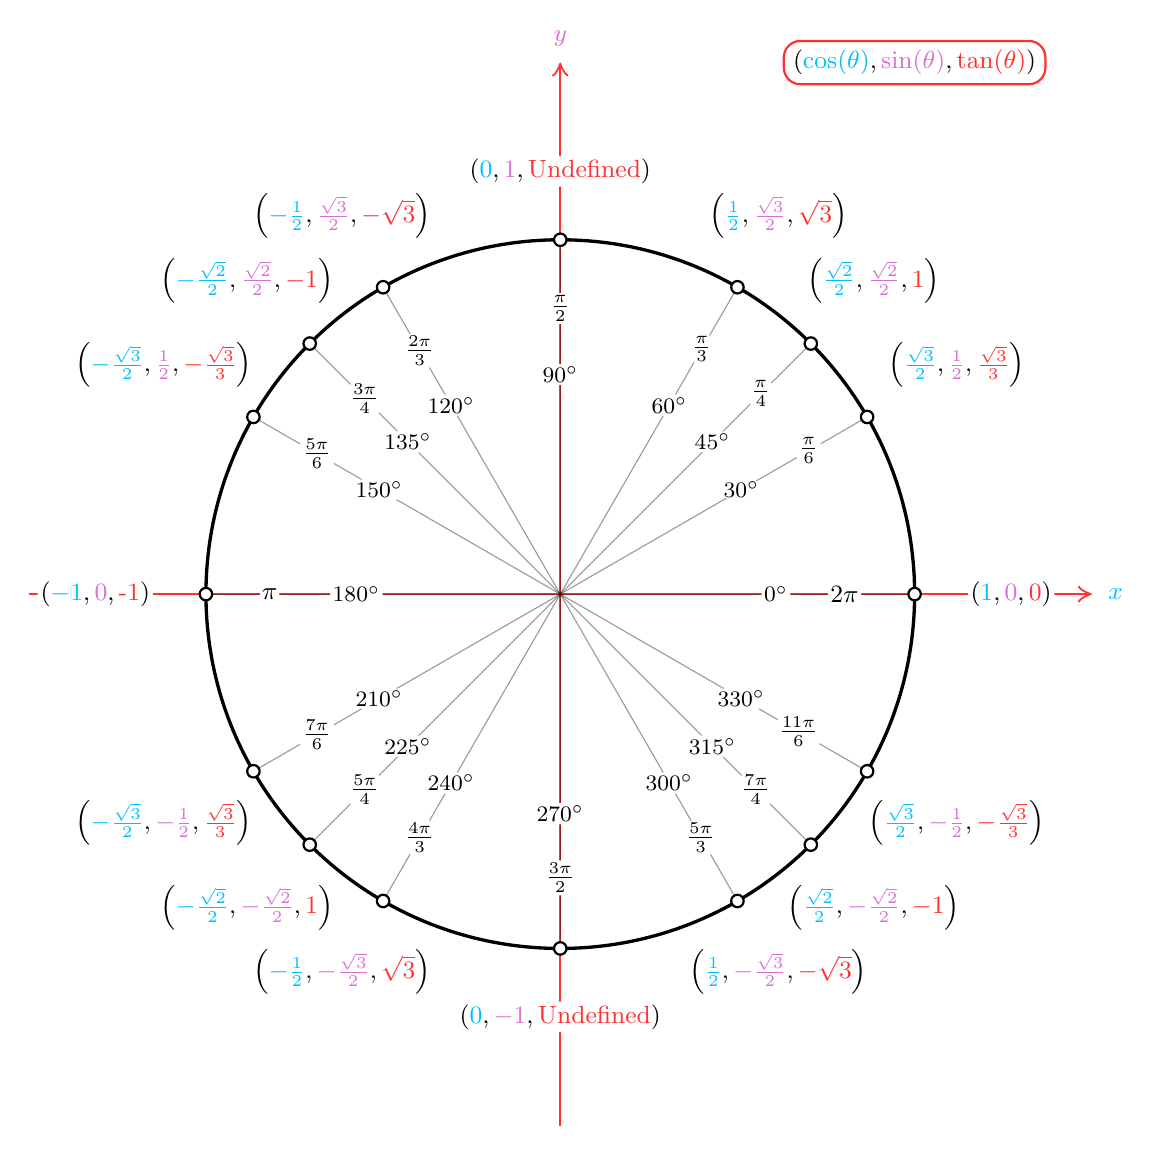
\begin{tikzpicture}[scale=4.5, font=\small]
    \definecolor{r}{HTML}{ff3030}
    \definecolor{b}{HTML}{00bfff}
    \definecolor{o}{HTML}{DA70D6}
    \def\angles{
        0/2\pi/1/0/0,
        30/\frac{\pi}{6}/\frac{\sqrt{3}}{2}/\frac{1}{2}/\frac{\sqrt{3}}{3},
        45/\frac{\pi}{4}/\frac{\sqrt{2}}{2}/\frac{\sqrt{2}}{2}/1,
        60/\frac{\pi}{3}/\frac{1}{2}/\frac{\sqrt{3}}{2}/\sqrt{3},
        90/\frac{\pi}{2}/0/1/\text{Undefined},
        120/\frac{2\pi}{3}/-\frac{1}{2}/\frac{\sqrt{3}}{2}/-\sqrt{3},
        135/\frac{3\pi}{4}/-\frac{\sqrt{2}}{2}/\frac{\sqrt{2}}{2}/-1,
        150/\frac{5\pi}{6}/-\frac{\sqrt{3}}{2}/\frac{1}{2}/-\frac{\sqrt{3}}{3},
        180/\pi/-1/0/\text{-1},
        210/\frac{7\pi}{6}/-\frac{\sqrt{3}}{2}/-\frac{1}{2}/\frac{\sqrt{3}}{3},
        225/\frac{5\pi}{4}/-\frac{\sqrt{2}}{2}/-\frac{\sqrt{2}}{2}/1,
        240/\frac{4\pi}{3}/-\frac{1}{2}/-\frac{\sqrt{3}}{2}/\sqrt{3},
        270/\frac{3\pi}{2}/0/-1/\text{Undefined},
        300/\frac{5\pi}{3}/\frac{1}{2}/-\frac{\sqrt{3}}{2}/-\sqrt{3},
        315/\frac{7\pi}{4}/\frac{\sqrt{2}}{2}/-\frac{\sqrt{2}}{2}/-1,
        330/\frac{11\pi}{6}/\frac{\sqrt{3}}{2}/-\frac{1}{2}/-\frac{\sqrt{3}}{3}
    }
    \begin{scope}[every node/.style={inner sep=1pt, outer sep=0pt}]
        \foreach \a/\at/\x/\y/\t in \angles {
            \begin{pgfinterruptboundingbox}
                \node (x) at (\a : 1.15) [anchor=\a-180] {\phantom{$\textstyle\left({\color{b} \x}, {\color{o} \y}, {\color{r} \t}\right)$}};
                \clip [rounded corners] (x.south west) rectangle (x.north east) (-1.6, -1.6) -- (1.6, -1.6) -- (1.6, 1.6) -- (-1.6, 1.6) -- cycle;
                \node (x) at (\a : 0.85) [anchor=\a] {\phantom{$\textstyle\at$}};
                \clip [rounded corners] (x.south west) rectangle (x.north east) (-1.6, -1.6) -- (1.6, -1.6) -- (1.6, 1.6) -- (-1.6, 1.6) -- cycle;
                \node (x) at (\a : 0.65) [anchor=\a, font=\footnotesize] {\phantom{$\textstyle\a^\circ$}};
                \clip [rounded corners] (x.south west) rectangle (x.north east) (-1.6, -1.6) -- (1.6, -1.6) -- (1.6, 1.6) -- (-1.6, 1.6) -- cycle;
                \clip (\a : 1) circle [radius=.5pt] (-1.6, -1.6) -- (-1.6, 1.6) -- (1.6, 1.6) -- (1.6, -1.6) -- cycle;
            \end{pgfinterruptboundingbox}
        }

        \draw [r, thick] (-1.5, 0) edge [-{Classical TikZ Rightarrow[length=5pt, width=6pt]}] (1.5, 0) node at (1.5, 0) [right=5pt] {$\textstyle\color{b} x$}
        (0, -1.5) edge [-{Classical TikZ Rightarrow[length=5pt, width=6pt]}] (0, 1.5) node at (0, 1.5) [above=5pt] {$\textstyle\color{o} y$};
        \draw [very thick] (0, 0) circle [radius=1];

        \foreach \a/\at/\x/\y/\t in \angles { \draw [opacity=.4] (0, 0) -- (\a : 1); }
    \end{scope}

    \scoped [every node/.style={inner sep=1pt, outer sep=0pt}] {
        \foreach \a/\at/\x/\y/\t in \angles {
            \node at (\a : 1.15) [anchor=\a-180, rounded corners] {$\textstyle\left({\color{b} \x}, {\color{o} \y}, {\color{r} \t}\right)$};
            \node at (\a : 0.85) [anchor=\a, rounded corners] {$\textstyle\at$};
            \node at (\a : 0.65) [anchor=\a, rounded corners, font=\footnotesize] {$\textstyle\a^\circ$};
            \draw [thick] (\a : 1) circle [radius=.5pt];
        }
    }

    \node at (1, 1.5) [thick, draw=r, rounded corners=6pt] {$\textstyle\left({\color{b} \cos(\theta)}, {\color{o} \sin(\theta)}, {\color{r} \tan(\theta)}\right)$};
\end{tikzpicture}


\newpage
\section{Trigonometric Ratios for Special Angles}

\subsection{Special Angles}
In trigonometry, certain angles have special significance due to their simplicity and exact values. The primary special angles are 0°, 30°, 45°, 60°, and 90°.

\subsubsection*{0° (Zero Degrees)}
\begin{minipage}{0.5\textwidth}
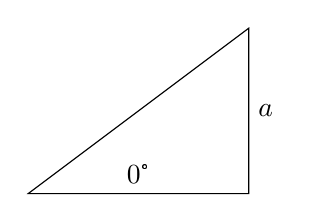
\begin{tikzpicture}[scale=0.7]
    \draw (0,0) -- (4,0) -- (4,3) -- cycle;
    \node[above] at (2,0) {0\textdegree};
    \node[right] at (4,1.5) {$a$};
\end{tikzpicture}
\end{minipage}%
\begin{minipage}{0.5\textwidth}
\[
\begin{aligned}
\sin(0^\circ) &= 0, \\
\cos(0^\circ) &= 1, \\
\tan(0^\circ) &= 0.
\end{aligned}
\]
\end{minipage}

\subsubsection*{30°}
\begin{minipage}{0.5\textwidth}
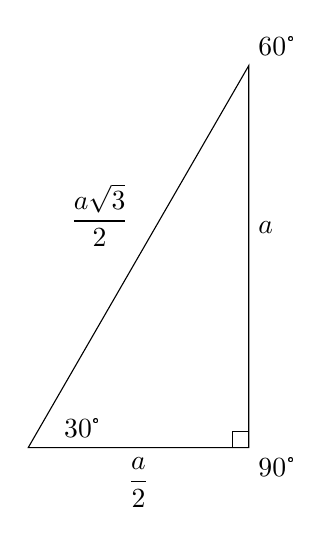
\begin{tikzpicture}[scale=0.7]
    \draw (0,0) -- (4,0) -- (4,{4*sqrt(3)}) -- cycle;
    \draw (3.7,0) -- (3.7,0.3) -- (4,0.3);
    \node[above left] at (1.5,0) {30\textdegree};
    \node[above right] at (4,{4*sqrt(3)}) {60\textdegree};
    \node[below right] at (4,0) {90\textdegree};
    \node[right] at (4,4) {$a$};
    \node[below] at (2,0) {$\dfrac{a}{2}$};
    \node[above left] at (2,{2*sqrt(3)}) {$\dfrac{a\sqrt{3}}{2}$};
\end{tikzpicture}
\end{minipage}%
\begin{minipage}{0.5\textwidth}
\[
\begin{aligned}
\sin(30^\circ) &= \dfrac{1}{2}, \\
\cos(30^\circ) &= \dfrac{\sqrt{3}}{2}, \\
\tan(30^\circ) &= \dfrac{1}{\sqrt{3}}.
\end{aligned}
\]
\end{minipage}

\subsubsection*{45°}
\begin{minipage}{0.5\textwidth}
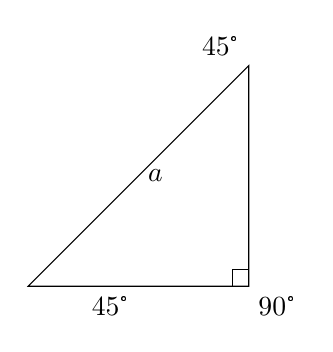
\begin{tikzpicture}[scale=0.7]
    \draw (0,0) -- (4,0) -- (4,4) -- cycle;
    \draw (3.7,0) -- (3.7,0.3) -- (4,0.3);
    \node[below left] at (2,0) {45\textdegree};
    \node[above left] at (4,4) {45\textdegree};
    \node[below right] at (4,0) {90\textdegree};
    \node[right] at (2,2) {$a$};
\end{tikzpicture}
\end{minipage}%
\begin{minipage}{0.5\textwidth}
\[
\begin{aligned}
\sin(45^\circ) &= \dfrac{\sqrt{2}}{2}, \\
\cos(45^\circ) &= \dfrac{\sqrt{2}}{2}, \\
\tan(45^\circ) &= 1.
\end{aligned}
\]
\end{minipage}

\subsubsection*{60°}
\begin{minipage}{0.5\textwidth}
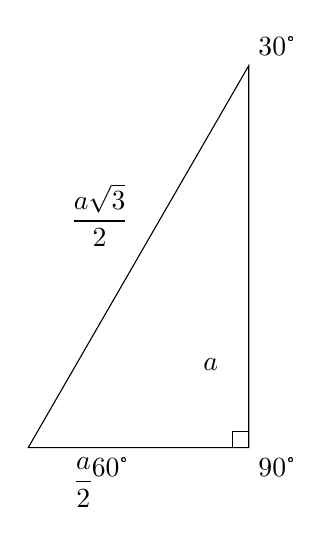
\begin{tikzpicture}[scale=0.7]
    \draw (0,0) -- (4,0) -- (4,{4*sqrt(3)}) -- cycle;
    \draw (3.7,0) -- (3.7,0.3) -- (4,0.3);
    \node[below left] at (2,0) {60\textdegree};
    \node[above right] at (4,{4*sqrt(3)}) {30\textdegree};
    \node[below right] at (4,0) {90\textdegree};
    \node[right] at (3,1.5) {$a$};
    \node[below] at (1,0) {$\dfrac{a}{2}$};
    \node[above left] at (2,{2*sqrt(3)}) {$\dfrac{a\sqrt{3}}{2}$};
\end{tikzpicture}
\end{minipage}%
\begin{minipage}{0.5\textwidth}
\[
\begin{aligned}
\sin(60^\circ) &= \dfrac{\sqrt{3}}{2}, \\
\cos(60^\circ) &= \dfrac{1}{2}, \\
\tan(60^\circ) &= \sqrt{3}.
\end{aligned}
\]
\end{minipage}

\subsubsection*{90°}
\begin{minipage}{0.5\textwidth}
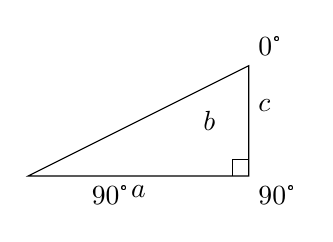
\begin{tikzpicture}[scale=0.7]
    \draw (0,0) -- (4,0) -- (4,2) -- cycle;
    \draw (3.7,0) -- (3.7,0.3) -- (4,0.3);
    \node[below left] at (2,0) {90\textdegree};
    \node[above right] at (4,2) {0\textdegree};
    \node[below right] at (4,0) {90\textdegree};
    \node[right] at (3,1) {$b$};
    \node[below] at (2,0) {$a$};
    \node[above right] at (4,1) {$c$};
\end{tikzpicture}
\end{minipage}%
\begin{minipage}{0.5\textwidth}
\[
\begin{aligned}
\sin(90^\circ) &= 1, \\
\cos(90^\circ) &= 0 \, (\text{undefined}), \\
\tan(90^\circ) &= \infty \, (\text{undefined}).
\end{aligned}
\]
\end{minipage}

\subsection{Coterminal Angles:}
Coterminal angles are angles that share the same initial and terminal sides but can differ by integer multiples of a full revolution (360° or $2\pi$ radians). Two angles $\theta$ and $\theta + 360n$ (where $n$ is an integer) are coterminal.

\subsection{Principal Angles:}
The principal angle is the smallest positive angle between the terminal side of an angle and the x-axis. For any angle $\theta$, the principal angle $\theta_p$ is given by:
\[ \theta_p = \theta - 360n \]
\newpage
\section{Trig identities}
An identity is an equation which is true for all values of the variable. 
\subsection{Reciprocal identity}
\begin{align*}
\csc(\theta) &= \frac{1}{\sin(\theta)} \\
\sec(\theta) &= \frac{1}{\cos(\theta)} \\
\cot(\theta) &= \frac{1}{\tan(\theta)}
\end{align*}
\subsection{Pythagorean identity}

$$\cos^2\theta +\sin^2\theta =1\\$$

\subsubsection*{Rearranging Pythagorean identity}
\begin{align*}
    \cos^2\theta +\sin^2\theta =1\\
    \cos^2\theta =1-\sin^2\theta\\
    \sin^2\theta=1-\cos^2\theta
\end{align*}
\subsection{Quotient identity:}
\[\tan\theta =\frac{\sin \theta}{\cos \theta} \quad \text{and } \quad \cot\theta=\frac{\cos\theta}{\sin\theta}\]
\section*{Steps to prove identities}
\begin{enumerate}
    \item Simplify one side at a time (Both sides is not allowed.)
    \item Start with more complicated side first.
    \item Simplify one side as much as you can, if you get stuck than switch to take other side.
    \item Converting everything into sine and cos is sometimes helpful.
    \item Use your intuition!
\end{enumerate}
\end{document}
